\documentclass{article}

\usepackage[paper=letterpaper,margin=2.5cm]{geometry} % Set Margins

%% Math and math fonts
\usepackage{amsmath, amsthm, amssymb, amsfonts}
\usepackage{bbm} % for \mathbbm{1}

% date
\usepackage[nodayofweek]{datetime}

% Color
\usepackage{color, xcolor}

% Misc
\usepackage{environ}  % \collect@body in asmmath
\usepackage{graphicx} % \includegraphics options
\usepackage{mdframed} % text boxes
\usepackage{indentfirst} % Indent first paragraph after section header
\usepackage[shortlabels]{enumitem} % Control enumerate items with [(a)]
\usepackage{comment} % Comments
\usepackage{fancyhdr} % Headers and footers

% Tables
\usepackage{array}

% Sub-figures and figure placement
\usepackage{caption}
\usepackage{subcaption}
\usepackage{float} 

% Graphing
\usepackage{pgfplots}
\pgfplotsset{compat=1.17}
\usepackage{tikz}

% Title Placement
\usepackage{titling}
\setlength{\droptitle}{-6em}

%set indent to 
\setlength{\parindent}{0pt}

% Hyper refs
\usepackage{hyperref}
\hypersetup{
    colorlinks=true,
    linkcolor=blue,
    urlcolor  = blue,
    filecolor=magenta,      
    urlcolor=blue,
    citecolor = blue,
    anchorcolor = blue
}

% % Citation management
\usepackage{natbib}
\bibliographystyle{abbrvnat}
\setcitestyle{authordate,open={(},close={)}}

\pagestyle{fancy}

\usepackage[paper=letterpaper,margin=2.5cm]{geometry} % Set Margins

%% Math and math fonts
\usepackage{amsmath, amsthm, amssymb, amsfonts}
\usepackage{bbm} % for \mathbbm{1}

% date
\usepackage[nodayofweek]{datetime}

% Color
\usepackage{color, xcolor}

% Misc
\usepackage{environ}  % \collect@body in asmmath
\usepackage{graphicx} % \includegraphics options
\usepackage{mdframed} % text boxes
\usepackage{indentfirst} % Indent first paragraph after section header
\usepackage[shortlabels]{enumitem} % Control enumerate items with [(a)]
\usepackage{comment} % Comments
\usepackage{fancyhdr} % Headers and footers

% Tables
\usepackage{array}

% Sub-figures and figure placement
\usepackage{caption}
\usepackage{subcaption}
\usepackage{float} 

% Graphing
\usepackage{pgfplots}
\pgfplotsset{compat=1.17}
\usepackage{tikz}

% Title Placement
\usepackage{titling}
\setlength{\droptitle}{-6em}

%set indent to 
\setlength{\parindent}{0pt}

% Hyper refs
\usepackage{hyperref}
\hypersetup{
    colorlinks=true,
    linkcolor=blue,
    urlcolor  = blue,
    filecolor=magenta,      
    urlcolor=blue,
    citecolor = blue,
    anchorcolor = blue
}

% % Citation management
\usepackage{natbib}
\bibliographystyle{abbrvnat}
\setcitestyle{authordate,open={(},close={)}}

% ----------------------------------------
% TITLE
% ----------------------------------------

\pagestyle{empty}

\lhead{Creel}
\chead{Week Five}
\rhead{AMES}

\title{AMES Class Notes -- Week Five, Day 2}
\author{Andie Creel}

\begin{document}
\maketitle

\section{Total Derivatives}
Total derivative in a function is equal to the sum of the partials multiplied by the change. 

Consider the function $ F = f(x,y)$. We can get our partial derivatives. Recall that when we take a partial derivative wrt $x$, we're holding $y$ constant.
\begin{align}
    \frac{\partial f}{\partial x} = f_x\\
    \frac{\partial f}{\partial y} = f_y
\end{align}

Now consider how we would calculate the change in $F$ if both $x$ and $y$ changed. We'd need to get a full derivative, 

\begin{align}
    df &= f_x dx + f_y dy \\
    &= \frac{\partial f}{\partial x} dx + \frac{\partial f}{\partial y} dy\\
    \Delta f = &= \frac{\partial f}{\partial x} \Delta x + \frac{\partial f}{\partial y} \Delta y
\end{align}
These are all equivalent ways of writing the full derivative. 


\subsection{Implicit Function Theorem (envelope theorem in econ)}

\begin{figure}[htp]
    \centering
        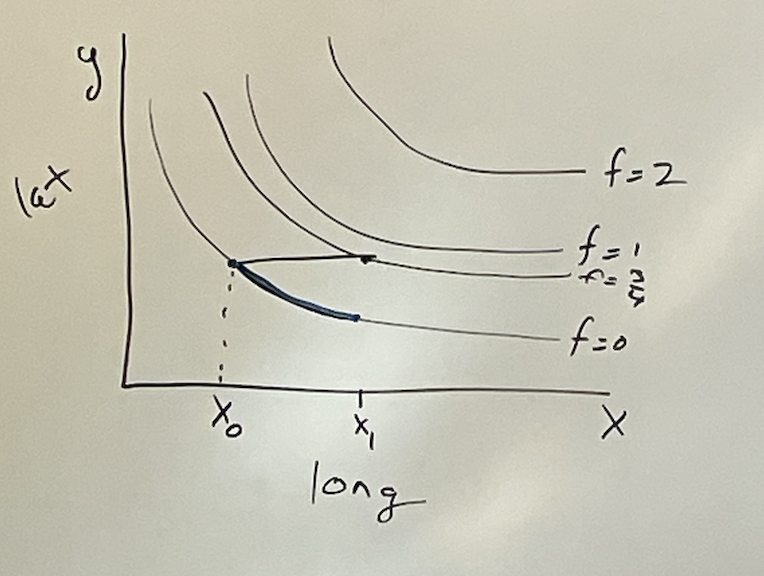
\includegraphics[width=0.5\textwidth]{Screen Shot 2023-09-27 at 10.59.32 AM.png}
    % \caption{convex and concave }
    % \label{fig:sample}
\end{figure}

Now consider if you want to stay on one level set. For example, if you wan to stay on a contour line or on a utility level. That would mean we want $F$ to stay the same, $df = \Delta f = 0$. 

\begin{align}
    d f = \frac{\partial f}{\partial x} dx + \frac{\partial f}{\partial y} dy &= 0 \implies \\
    dy \frac{\partial f}{\partial y} dy &= - dx \frac{\partial f}{\partial x} \implies \\
    \frac{d y}{dx} &= \frac{- \frac{\partial f}{\partial x}}{\frac{\partial f}{\partial y}} \label{imp_func}
\end{align}

Equation \ref{imp_func} is the implicit function theorem. What equation \ref{imp_func} tells us is "if I want to stay on the same level set, and I change $x$, how do I need to change $y$ in order to stay on that level set".\\


\textbf{The envelope theorem} is a special case of the implicit function theorem when first derivatives are set to zero. This leads to math simplifying because we can say that, at the optimum, a bunch of derivatives will equal zero. 

\section{Taylor Series}

We know that straight lines are good approximators because a line is a conditional mean, and means are good at minimizing error.\\

Series are good approximators of sequences of numbers, because series are functions. \\

A \textbf{Taylor Series} is an extremely useful series for approximating the relationship of sequence of numbers (data is a sequence of numbers). Taylor series underpins a lot of the math we do today, particularly for any relationship that isn't linear. 

\begin{align}
    f(x) = f(a) + \frac{f'(a)}{1!}(x-a)^1 + \frac{f''(a)}{2!}(x-a)^2 + \frac{f'''(a)}{3!}(x-a)^3 + ... + \frac{f^k(a)}{k!}(x-a)^k + R
\end{align}
where $R$ is the residual.\\


\subsection{0th order Taylor Series}
Consider a 0th order taylor series: it would be a mean aka just a flat line equal to $f(a)$. \\

If you're only looking at the means of a dataset, that means you're doing a 0th order taylor approximation.

\subsection{First order Taylor Series}

Consider a first order taylor series: 
\begin{align}
    f(x) &= f(a) + \frac{f'(a)}{1!}(x-a)^1 \\
    &= A + B (x-a) \\
    &= A -aB + Bx\\
    &= m + Bx
\end{align}
It's a line with a slope. A first order Taylor series is a linear approximation. Linear regression is a first order Taylor approximation. \\

\subsection{Discussion of models}
Any Taylor Series approximation is a model. If someone says "I don't do models, let's only do means" they actually \textit{are} suggesting a model. A mean is a model, it's a zero order Taylor Series approximation! 

Higher order Taylor Series will approximate an underlying function better than a lower order. \textit{However,} we do not always have enough data to fit a higher order Taylor series because it would require more estimating parameters and your data set may not have enough power (aka enough data) to do so. 

\subsection{Example: Logistic growth}
Consider the logistic growth function: 
\begin{align}
    G(N) = rN (1 - \frac{N}{K})
\end{align}

What would we get if we "taylor expanded" this function? Let's work with the per capital growth rate
\begin{align}
    \frac{G(N)}{N} = r(1 - \frac{N}{K}) \label{per_cap}
\end{align}
and see if we can use a Taylor series that would approximate this right hand side equation

\begin{align}
    \frac{G(N)}{N} &\approx G(a) + G'(a) (N-a)\\
    &\approx G(a) + G'(a)N - G'(a)a \\
    & \approx G(a) - G'(a)a + G'(a) N
\end{align}

Let $r =  - G'(a)a$.
\begin{align}
    & \approx r + G(a) + G'(a) N
\end{align}

Let $G(a) = 0$  and rename $G'(a) = \frac{-r}{K}$

\begin{align}
    &\approx r + \frac{-r}{K}N\\
    &\approx r(1 - \frac{N}{K}) \label{approx}
\end{align}

And now we've shown that \ref{approx} is equivalent to \ref{per_cap}. Which means we've shown that we can derive the logistic growth equation using a Taylor series approximation.

\subsection{Exercise}
What's is $\sqrt{10}$? The function of consideration is
\begin{align}
    f(x) = \sqrt{x} = x^{\frac{1}{2}}.
\end{align}

We're interested when $x = 10$. Let's do a \textbf{0th order taylor series approximation}: 

\begin{align}
    f(x) = f(a)
\end{align}

what should we choose $a$ to be? Let's choose $a = 9$ because 9 is close to 10. 

\begin{align}
    f(10) & \approx f(a) \\
    & \approx f(9)\\
    & \approx \sqrt{9}\\
    & \approx 3
\end{align}

Let's do a \textbf{first order taylor series approximation} 
\begin{align}
    f(x) &\approx f(a) + \frac{f'(a)}{1!}(x-a)^1\\
    f(10) &\approx f(9) +  \frac{f'(9)}{1!}(10-9)^1\\
    &\approx \sqrt{9} + \frac{1}{2}(9)^{-1/2}\\
    &\approx 3 + \frac{1}{2}\frac{1}{(9)^{1/2}}\\
    &\approx 3 \frac{1}{6}
\end{align}

You could then do a second order taylor series approximation and get even closer.


\end{document}